\textbf{S-LLMs Evaluated}. SimBench is demonstrated in conjunction with benchmarking a set of 33 S-LLMs,
encompassing both open- and closed-source models of various sizes, architectures, and family.
For closed-source models, we include commercial S-LLMs, such as \textbf{gpt-4.1-nano} and \textbf{o4-mini}
from OpenAI, as well as \textbf{Claude 4.0 Sonnet} from Anthropic, and \textbf{Gemini 2.5pro} from Google.
The open-source models evaluated include from the \textbf{LLaMA-3.1} family (8B, 70B, 405B) to the \textbf{LLaMA-4} family (400B, 109B).
We included specialized models like \textbf{codellama-70B}, \textbf{codestral-22B}, \textbf{CodeGemma-7B}, and also the mamba class \textbf{mamba-codestral-7b} model,
fine-tuned for code generation. We also considered S-LLMs that have been trained on a mix of general and 
domain-specific data, e.g., \textbf{Gemma-2} (2B, 9B, 27B) and \textbf{Mistral} (12b, 8x7b, 8x22B). 
Additionally, models such as \textbf{Phi-3} (3.8B, 7B, 14B) and \textbf{Mixtral} (8x7B, 8x22B) 
are included to explore the impact of different scales and training regimes on their ability to perform in 
multi-turn setups. 

In terms of generation settings, unless otherwise specified, we sample S-LLM outputs with temperature $=0.6$ and top-$p=0.9$ using a fixed prompt wrapper shared across models. We exclude base (non-instruction-tuned) code models to focus on instruction-following behavior. For the judge (J-LLM), we use temperature $=0.2$ and top-$p=0.7$ to reduce scoring variance. The judge prompt is calibrated once and then frozen for all models and tasks. All raw data for evaluation of models under three types of metrics (similarity, J-LLM, and execution-based) are included in the repository.

\begin{comment}
\begin{table*}[htbp]
  \centering
  \resizebox{\textwidth}{!}{%
  \begin{tabular}{lccccc c}
  \toprule
  \textbf{Model} & \textbf{Company} & \textbf{Open Weights} & \textbf{Size} & \textbf{Release} & \textbf{Reasoning} & \textbf{J-LLM-Ref-Doc} \\
  \midrule
  claude-4-sonnet-20250514 & Anthropic & -- & -- & 2025-Q2 & \checkmark & 49 \\
  o3 & OpenAI & -- & -- & 2025-Q2 & \checkmark & 46 \\
  claude-3-7-sonnet-20250219 & Anthropic & -- & -- & 2025-Q1 & \checkmark & 43 \\
  o4-mini & OpenAI & -- & -- & 2025-Q2 & \checkmark & 42 \\
  qwen3-235b-a22b & Alibaba & \checkmark & 235B & 2025-Q2 & \checkmark & 42 \\
  Gemini-2.5-pro & Google & -- & -- & 2025-Q2 & \checkmark & 41 \\
  gpt-4.1-mini & OpenAI & -- & -- & 2025-Q2 & -- & 41 \\
  gpt-4o-mini & OpenAI & -- & -- & 2024-Q3 & -- & 41 \\
  llama4-maverick & Meta & \checkmark & 400B & 2025-Q2 & -- & 41 \\
  llama4-scout & Meta & \checkmark & 109B & 2025-Q2 & -- & 41 \\
  llama-3.3-70b & Meta & \checkmark & 70B & 2024-Q4 & -- & 41 \\
  deepseek-r1-32b & DeepSeek & \checkmark & 32B & 2025-Q1 & \checkmark & 40 \\
  gpt-4.1-nano & OpenAI & -- & -- & 2025-Q2 & -- & 40 \\
  llama-3.1-70b & Meta & \checkmark & 70B & 2024-Q3 & -- & 40 \\
  gpt-4.1 & OpenAI & -- & -- & 2025-Q2 & -- & 39 \\
  Gemini-1.5-pro & Google & -- & -- & 2024-Q1 & -- & 39 \\
  codestral-22b-v0.1 & Mistral & \checkmark & 22B & 2024-Q2 & -- & 39 \\
  llama-3.1-405b & Meta & \checkmark & 405B & 2024-Q3 & -- & 39 \\
  mixtral-8x22b-v0.1 & Mistral & \checkmark & 176B (8$\times$22B) & 2024-Q2 & -- & 39 \\
  llama-3.1-8b & Meta & \checkmark & 8B & 2024-Q3 & -- & 38 \\
  mistral-nemo-12b & Mistral & \checkmark & 12B & 2024-Q3 & -- & 38 \\
  gemma-2-27b & Google & \checkmark & 27B & 2024-Q2 & -- & 36 \\
  mixtral-8x7b-v0.1 & Mistral & \checkmark & 46.7B (8$\times$7B) & 2023-Q4 & -- & 36 \\
  claude-3-5-sonnet & Anthropic & -- & -- & 2024-Q2 & -- & 34 \\
  deepseek-r1-8b & DeepSeek & \checkmark & 8B & 2025-Q1 & \checkmark & 34 \\
  gpt-4o & OpenAI & -- & -- & 2024-Q2 & -- & 34 \\
  nemotron-4-340b & NVIDIA & \checkmark & 340B & 2024-Q2 & -- & 34 \\
  gemma-2-9b & Google & \checkmark & 9B & 2024-Q2 & -- & 32 \\
  gemma-2-2b & Google & \checkmark & 2B & 2024-Q2 & -- & 30 \\
  mamba-codestral-7b-v0.1 & Mistral & \checkmark & 7B & 2024-Q3 & -- & 30 \\
  gemma-3-1b & Google & \checkmark & 1B & 2025-Q1 & -- & 26 \\
  phi-3-mini-128k & Microsoft & \checkmark & 3.8B & 2024-Q2 & -- & 25 \\
  phi-3-medium-128k & Microsoft & \checkmark & 14B & 2024-Q2 & -- & 21 \\
  \bottomrule
  \end{tabular}
  }
  \caption{Overview of pretrained S-LLMs evaluated in this study. ``Open Weights'' indicates whether model weights are publicly available. ``Reasoning'' indicates models explicitly positioned or configured for deliberate reasoning by their providers. ``Perf'' reports the overall J-LLM Ref Doc average score (Table~\ref{tab:pretrain_models_performance}). Models are ordered by \textbf{J-LLM-Ref-Doc}.}
  \vspace{-10pt}
  \label{tab:model_info}
\end{table*}
\end{comment}


\subsection{Historical Trends in S-LLM Performance on SimBench}

To evaluate whether S-LLM simulation code generation performance has improved across successive six-month intervals, we analyze the relationship between model release dates and J-LLM scores. Figure~\ref{fig:temporal_trend} plots the average of the three modalities of J-LLM scores (J-LLM\_Ref\_Doc, J-LLM\_Ref, and J-LLM\_Doc) against release dates for all 33 evaluated models. 
A clear positive trend emerges: models released more recently demonstrate stronger performance on SimBench tasks. 

Computing correlation coefficient yields $\rho = 0.624$ ($p < 0.001$), indicating a significant temporal improvement in simulation code generation capabilities. Several notable observations emerge from this temporal analysis. First, the variance in performance has increased over time: while early models (2023 Q4-2024 Q3) cluster in the 30-40 score range, recent models (2025 Q1-Q3) span from 40 to 49, suggesting both continued improvement of frontier models and diversification of capabilities across different model families. Second, reasoning-enhanced models released in 2025 Q1-Q2 consistently occupy the upper performance tier, with Claude-4-Sonnet, o3, and Claude-3.7-Sonnet achieving the top three positions. Third, model scale alone does not guarantee superior performance. Indeed, several smaller recent models (e.g., gpt-4.1-nano, gpt-4.1-mini) outperform earlier large-scale models (e.g., Nemotron-4-340B, Llama-3.1-405B), highlighting the importance of architectural innovations and training methodologies beyond parameter count.

The temporal trend analysis indicates that SimBench is sensitive to meaningful differences in model capability and that the field is making measurable progress in simulation-focused code generation. This trajectory suggests that continued advances, especially improved long-horizon code editing, stronger tool use, and better simulator-specific grounding, should translate into higher performance on complex multi-turn simulation tasks.

\begin{figure*}[htbp]
\centering
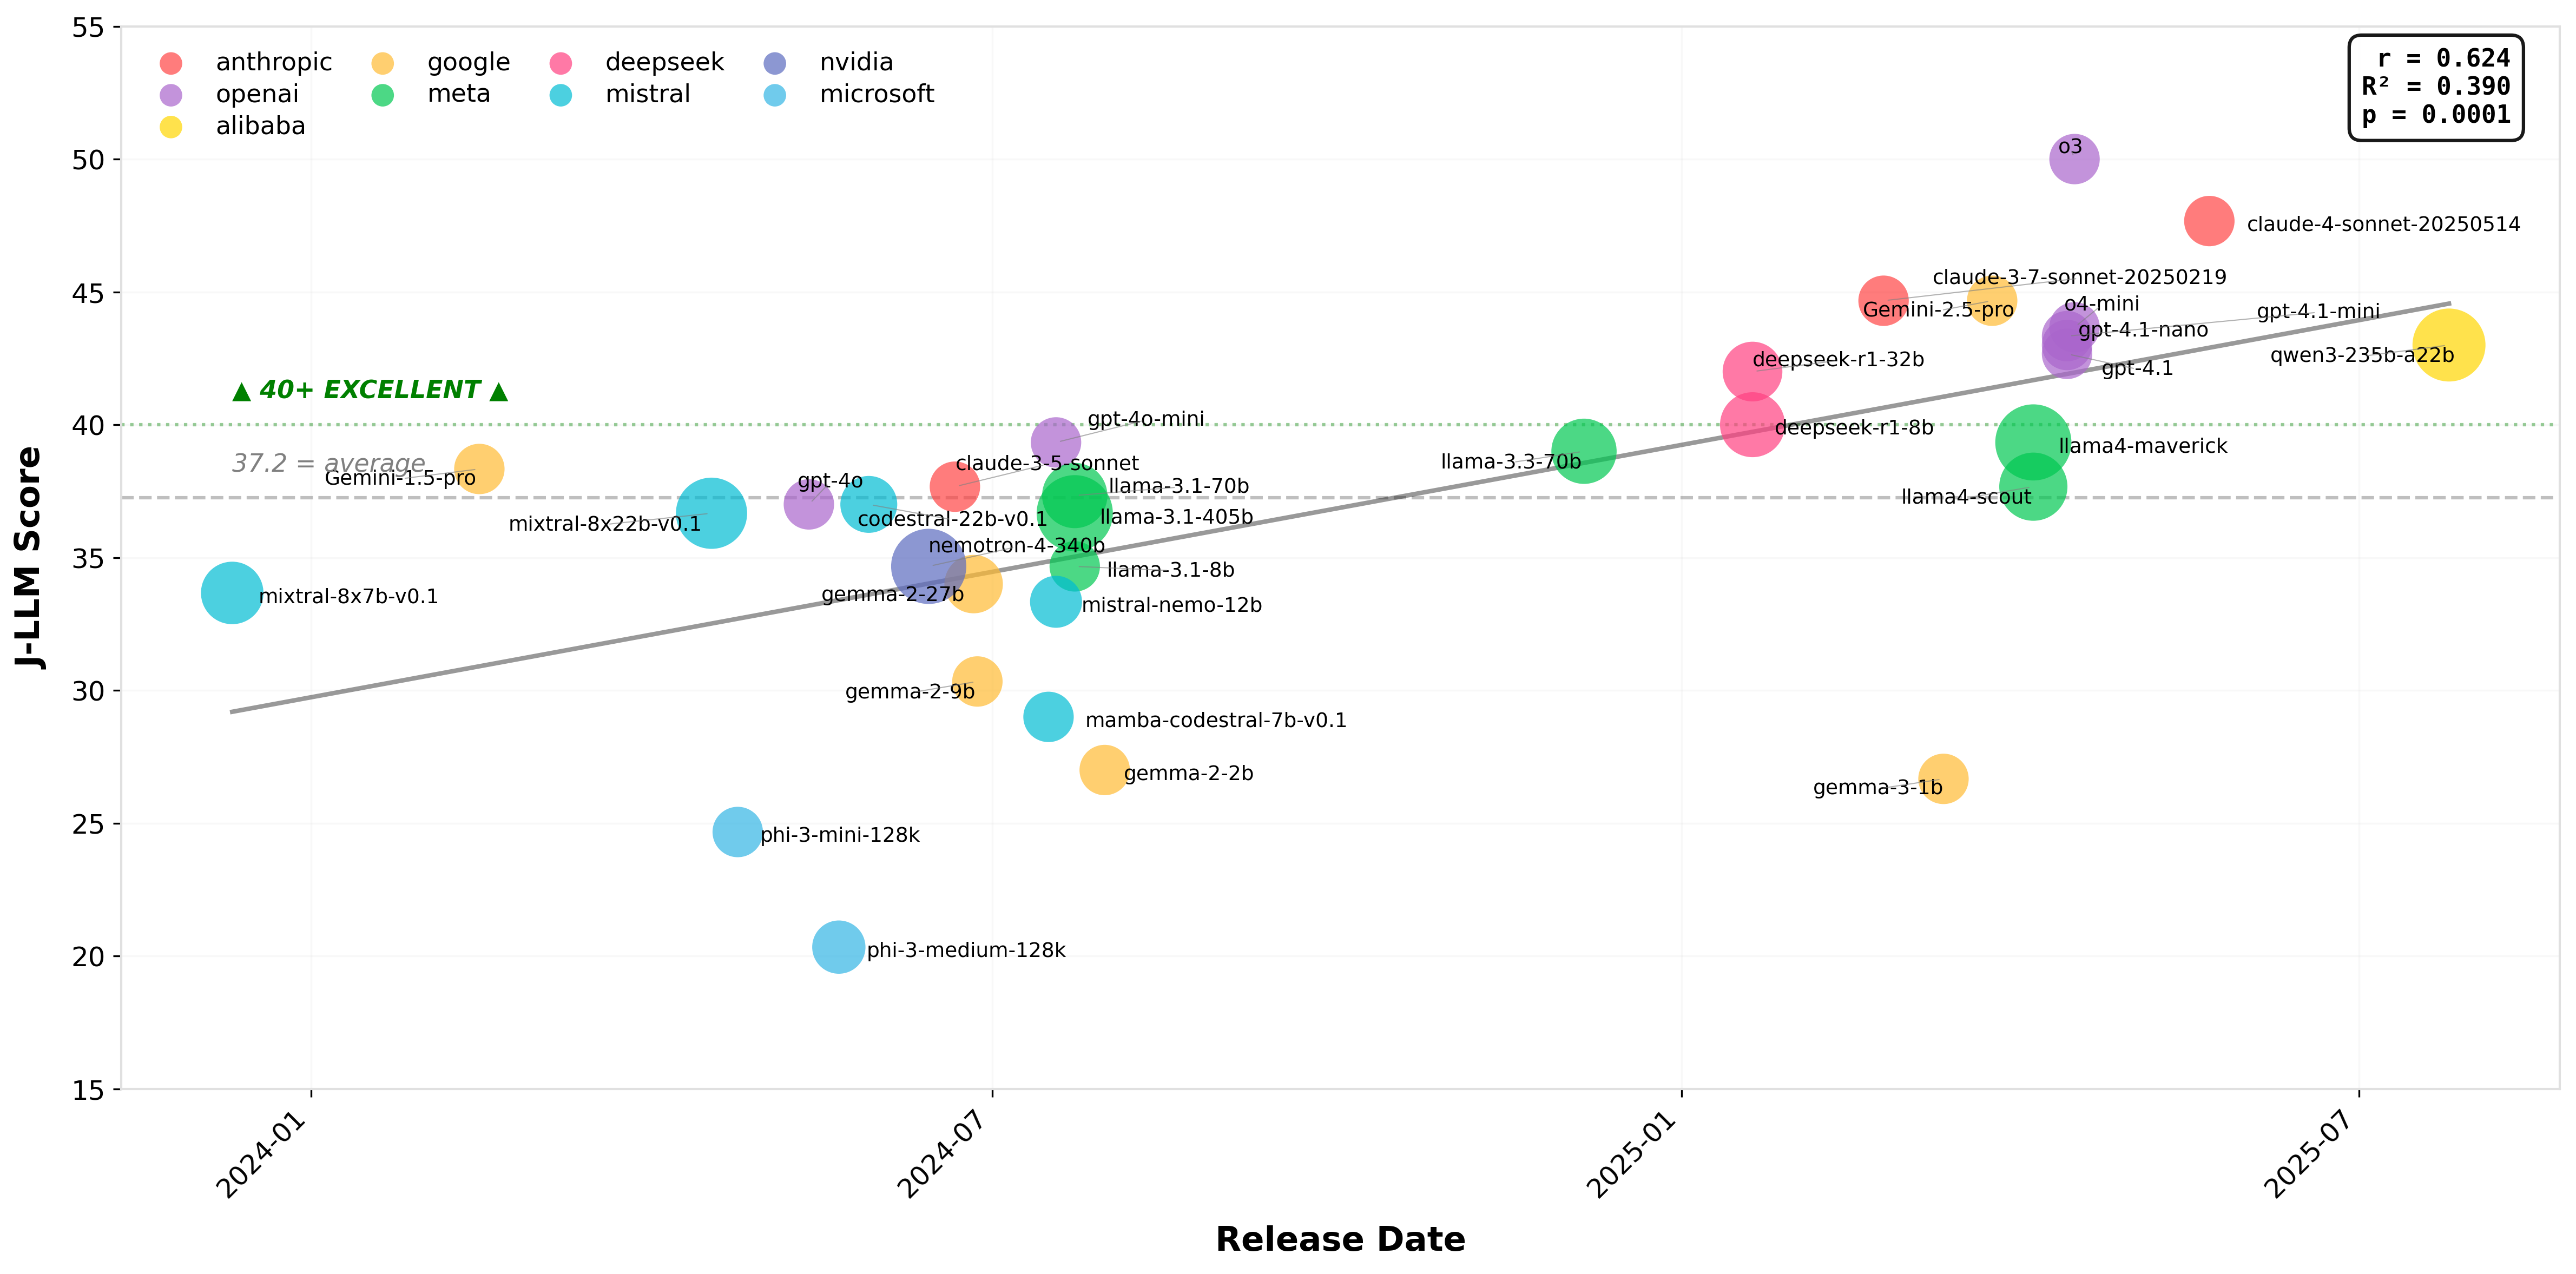
\includegraphics[width=\textwidth]{images/jllm_vs_exact_dates.png}
\caption{Temporal evolution of S-LLM performance on SimBench. Y-axis is the average of three modalities of J-LLM scores, they are plotted against model release dates, 
showing a positive trend ($\rho = 0.624$, $p < 0.001$).}
\label{fig:temporal_trend}
\end{figure*}

\begin{table*}[htbp]
  \centering
  \resizebox{\textwidth}{!}{%
  \begin{tabular}{lccccc ccc}
  \toprule
  \textbf{Model} & \textbf{Company} & \textbf{Open Weights} & \textbf{Size} & \textbf{Release} & \textbf{Reasoning} & \textbf{J-LLM-Ref-Doc} & \textbf{J-LLM-Ref} & \textbf{J-LLM-Doc} \\
  \midrule
  claude-4-sonnet & Anthropic & -- & -- & 2025-Q2 & \checkmark & 49 & 39 & 55 \\
  o3 & OpenAI & -- & -- & 2025-Q2 & \checkmark & 46 & 37 & 67 \\
  claude-3-7-sonnet & Anthropic & -- & -- & 2025-Q1 & \checkmark & 43 & 36 & 55 \\
  o4-mini & OpenAI & -- & -- & 2025-Q2 & \checkmark & 42 & 35 & 54 \\
  qwen3-235b-a22b & Alibaba & \checkmark & 235B & 2025-Q2 & \checkmark & 42 & 32 & 55 \\
  Gemini-2.5-pro & Google & -- & -- & 2025-Q2 & \checkmark & 41 & 31 & 62 \\
  gpt-4.1-mini & OpenAI & -- & -- & 2025-Q2 & -- & 41 & 34 & 55 \\
  gpt-4o-mini & OpenAI & -- & -- & 2024-Q3 & -- & 41 & 28 & 49 \\
  llama4-maverick & Meta & \checkmark & 400B & 2025-Q2 & -- & 41 & 33 & 44 \\
  llama4-scout & Meta & \checkmark & 109B & 2025-Q2 & -- & 41 & 34 & 38 \\
  llama-3.3-70b & Meta & \checkmark & 70B & 2024-Q4 & -- & 41 & 34 & 42 \\
  deepseek-r1-32b & DeepSeek & \checkmark & 32B & 2025-Q1 & \checkmark & 40 & 32 & 54 \\
  gpt-4.1-nano & OpenAI & -- & -- & 2025-Q2 & -- & 40 & 34 & 55 \\
  llama-3.1-70b & Meta & \checkmark & 70B & 2024-Q3 & -- & 40 & 33 & 39 \\
  gpt-4.1 & OpenAI & -- & -- & 2025-Q2 & -- & 39 & 34 & 55 \\
  Gemini-1.5-pro & Google & -- & -- & 2024-Q1 & -- & 39 & 33 & 43 \\
  codestral-22b-v0.1 & Mistral & \checkmark & 22B & 2024-Q2 & -- & 39 & 32 & 40 \\
  llama-3.1-405b & Meta & \checkmark & 405B & 2024-Q3 & -- & 39 & 33 & 38 \\
  mixtral-8x22b-v0.1 & Mistral & \checkmark & 176B (8$\times$22B) & 2024-Q2 & -- & 39 & 34 & 37 \\
  llama-3.1-8b & Meta & \checkmark & 8B & 2024-Q3 & -- & 38 & 31 & 35 \\
  mistral-nemo-12b & Mistral & \checkmark & 12B & 2024-Q3 & -- & 38 & 30 & 32 \\
  gemma-2-27b & Google & \checkmark & 27B & 2024-Q2 & -- & 36 & 29 & 37 \\
  mixtral-8x7b-v0.1 & Mistral & \checkmark & 46.7B (8$\times$7B) & 2023-Q4 & -- & 36 & 34 & 31 \\
  claude-3-5-sonnet & Anthropic & -- & -- & 2024-Q2 & -- & 34 & 26 & 53 \\
  deepseek-r1-8b & DeepSeek & \checkmark & 8B & 2025-Q1 & \checkmark & 34 & 32 & 54 \\
  gpt-4o & OpenAI & -- & -- & 2024-Q2 & -- & 34 & 28 & 49 \\
  nemotron-4-340b & NVIDIA & \checkmark & 340B & 2024-Q2 & -- & 34 & 30 & 40 \\
  gemma-2-9b & Google & \checkmark & 9B & 2024-Q2 & -- & 32 & 29 & 30 \\
  gemma-2-2b & Google & \checkmark & 2B & 2024-Q2 & -- & 30 & 27 & 24 \\
  mamba-codestral-7b-v0.1 & Mistral & \checkmark & 7B & 2024-Q3 & -- & 30 & 29 & 28 \\
  gemma-3-1b & Google & \checkmark & 1B & 2025-Q1 & -- & 26 & 26 & 28 \\
  phi-3-mini-128k & Microsoft & \checkmark & 3.8B & 2024-Q2 & -- & 25 & 25 & 24 \\
  phi-3-medium-128k & Microsoft & \checkmark & 14B & 2024-Q2 & -- & 21 & 20 & 20 \\
  \bottomrule
  \end{tabular}
  }
  \caption{Pretrained models evaluated in this study and their SimBench performance. ``Open Weights'' indicates whether model parameters are publicly released. ``Release'' reports the provider-announced release quarter. ``Reasoning'' marks models that providers explicitly market or expose as deliberate-reasoning variants. ``J-LLM-Ref-Doc'', ``J-LLM-Ref'', and ``J-LLM-Doc'' are rubric-based judge scores averaged over all task families and all three turns under three evaluation conditions (reference+documentation, reference-only, documentation-only). Models are ordered by ``J-LLM-Ref-Doc''.}
  \label{tab:model_info}
\end{table*}


\subsection{Robustness Analysis of J-LLM Metrics}


\noindent\textbf{Rubric-based J-LLM scores are robust to the choice of judge model and inference variability.}
To validate the robustness of our evaluation framework, we conducted cross-validation using three different J-LLM evaluators (GPT-4o-mini, GPT-4.1-nano, and GPT-4.1-mini) under the \textbf{J-LLM-Ref-Doc} modality, with three independent inference runs.

Table~\ref{tab:jllm_correlation} reports inter-evaluator agreement. All three evaluators exhibit high consistency, with Pearson correlations ranging from 0.8163 to 0.9489 (all $p < 0.001$). GPT-4.1-mini and GPT-4o-mini show near-perfect agreement ($r = 0.9489$), and all pairs maintain strong Spearman correlations (0.8455--0.9144), confirming consistent model rankings across evaluators.

\begin{table}[htbp]
\centering
\caption{Inter-evaluator correlation on Ref-Doc modality (all $p < 0.001$).}
\label{tab:jllm_correlation}
\begin{tabular}{lcc}
\toprule
\textbf{Evaluator Pair} & \textbf{Pearson $r$} & \textbf{Spearman $\rho$} \\
\midrule
GPT-4.1-mini vs GPT-4o-mini & 0.9489 & 0.9144 \\
GPT-4.1-mini vs GPT-4.1-nano & 0.8163 & 0.8455 \\
GPT-4.1-nano vs GPT-4o-mini & 0.8460 & 0.8905 \\
\bottomrule
\end{tabular}
\end{table}

Table~\ref{tab:jllm_statistics} summarizes the score distributions. Although the evaluators differ in absolute score levels, e.g., GPT-4.1-nano is the most lenient (mean 39.13) while GPT-4.1-mini is the most stringent (mean 32.34), the strong Pearson and Spearman correlations indicate robust cross-judge consistency. In particular, despite shifts in score calibration, the J-LLMs produce highly aligned relative rankings of generated DT solutions.

\begin{table}[htbp]
\centering
\caption{Score statistics for different J-LLMs under \textbf{J-LLM-Ref-Doc}.}
\label{tab:jllm_statistics}
\begin{tabular}{lcccc}
\toprule
\textbf{Evaluator} & \textbf{Mean} & \textbf{Std} & \textbf{Min} & \textbf{Max} \\
\midrule
GPT-4.1-mini & 32.34 & 6.59 & 14.35 & 40.62 \\
GPT-4.1-nano & 39.13 & 4.59 & 32.00 & 46.37 \\
GPT-4o-mini  & 36.00 & 5.33 & 21.75 & 40.99 \\
\bottomrule
\end{tabular}
\end{table}

Overall, these results show that the rubric-based framework yields consistent assessments across different J-LLM choices and across repeated inference runs, supporting reproducible and reliable evaluation. 

\medskip


{\noindentBold{Rubric-based J-LLM scores as practical proxies for Pass@1.}}
Execution-based correctness metrics such as Pass@1 provide the most direct validation of simulator-grade DT code, since they reflect whether the generated implementation is both syntactically valid and functionally correct in the simulator.
However, for complex multi-physics simulations, Pass@1 is costly to obtain: it requires expert assessment and/or extensive scenario-specific tests, which are difficult to author and may involve long runtimes.
A key goal of SimBench is therefore to provide an \emph{interpretable} judging signal that can serve as a practical surrogate for Pass@1 when exhaustive execution-based testing is infeasible.

We compare Pass@1 against three rubric-based J-LLM variants (Sec.~\ref{sec:modalities}): \textbf{J-LLM\_Ref\_Doc} (reference code + API excerpt), \textbf{J-LLM\_Ref} (reference code only), and \textbf{J-LLM\_Doc} (API excerpt only).
As additional baselines, we report an execution-based syntactic metric \textbf{Compile@1} and two commonly used similarity metrics, \textbf{CodeBLEU} and \textbf{ROUGE-LSUM}.
Table~\ref{tab:llm_metrics_final} summarizes the average metric values across all tasks for each S-LLM.

SimBench contains $N_{\text{sys}}=34$ physical systems, each evaluated under a fixed three-turn protocol, yielding $N_{\text{task}}=102$ turn-level tasks.
We evaluate a representative set of 19 widely used models, producing
$N_{\text{inst}} = 34 \times 3 \times 19 = 1938$ matched (model, system, turn) instances with 7 metric values, total $1938 \times 7 = 13,566$ data points; see Table~\ref{tab:llm_metrics_final}.
Pass@1 is assessed by human Chrono experts, whereas Compile@1 is computed automatically.
To quantify whether rubric-based J-LLM scores track execution-based correctness, we compute Spearman rank correlations over the $N_{\text{inst}}$ matched instances across metrics.
The resulting correlation matrix is shown in Fig.~\ref{fig:correlation_matrix}.

Considering correlation with Pass@1, \textbf{J-LLM\_Ref\_Doc} achieves the strongest association ($\rho=0.69$), followed by \textbf{J-LLM\_Ref} ($\rho=0.57$) and \textbf{Compile@1} ($\rho=0.49$).
We emphasize that Compile@1 is already a strong and widely used evaluation signal in code generation, and it is often used as a reward signal in RLVR-style training.
The fact that \textbf{J-LLM\_Ref\_Doc} exhibits an even stronger correlation with Pass@1 than Compile@1 supports its effectiveness as a proxy for functional correctness.
In contrast, similarity metrics correlate more weakly with Pass@1 (CodeBLEU: $\rho=0.42$; ROUGE-LSUM: $\rho=0.15$), suggesting that surface-form overlap is insufficient to capture simulator correctness in DT generation.
We also observe that \textbf{J-LLM\_Doc} correlates strongly with similarity metrics (CodeBLEU: $\rho=0.79$; ROUGE-LSUM: $\rho=0.94$), suggesting that, under our prompting setup, a doc-only judge may behave similarly to surface-form similarity measures. Nevertheless, this can still be valuable, since similarity metrics require reference code, whereas \textbf{J-LLM\_Doc} does not.
Overall, reference-conditioned rubric judging (\textbf{J-LLM\_Ref\_Doc} and \textbf{J-LLM\_Ref}) provides a substantially stronger indicator of Pass@1 than compile- or similarity-based alternatives, supporting its use as an interpretable benchmark metric for simulator-grade DT code.



\begin{table}[htbp]
    \centering
    \resizebox{0.5\textwidth}{!}{%
    \begin{tabular}{|l|c|c|c|c|c|c|c|}
    \hline
	{\tiny \textbf{S-LLM} $\downarrow$  $|$ \textbf{Metric} $\rightarrow$} & {\tiny \textbf{Pass@1}} & {\tiny \textbf{J-LLM\_Ref\_Doc}} & {\tiny \textbf{J-LLM\_Ref}} & {\tiny \textbf{J-LLM\_Doc}} & {\tiny \textbf{ROUGE-LSUM}} & {\tiny \textbf{CodeBLEU}} & {\tiny \textbf{Compile@1}}\\
    \hline
    gpt-4o-mini & 12.8\% & 41.6 & 34.1 & 43.7 & 0.723 & 0.610 & 19.6\% \\
    codestral-22b & 9.8\% & 37.9 & 32.4 & 39.7 & 0.699 & 0.608 & 20.6\% \\
    mixtral-8x22b & 7.8\% & 38.9 & 33.8 & 36.9 & 0.667 & 0.589 & 19.6\% \\
    claude-3.5-sonnet & 6.8\% & 33.7 & 25.9 & 52.8 & 0.757 & 0.591 & 7.8\%\\
    Gemini-1.5-Pro & 6.8\% & 39.2 & 32.9 & 42.7 & 0.727 & 0.609 & 7.8\% \\
    mixtral-8x7b & 6.8\% & 37.7 & 34.4 & 30.7 & 0.624 & 0.508 & 14.7\% \\
    llama-3.1-405b & 6.8\%& 39.0 & 33.1 & 38.0 & 0.720 & 0.619 & 19.6\% \\
    mistral-nemo-12b & 6.8\% & 36.4 & 29.7 & 31.8 & 0.648 & 0.552 & 17.6\% \\
    llama-3.1-8b & 4.9\% & 37.6 & 31.1 & 34.5 & 0.656 & 0.571 & 13.7\% \\
    gemma-2-27b & 4.9\% & 37.4 & 29.3 & 36.5 & 0.710 & 0.590 & 20.6\% \\
    llama-3.1-70b & 3.9\% & 39.7 & 33.3 & 39.4 & 0.710 & 0.540 & 8.8\% \\
    gemma-2-9b & 3.9\% & 33.5 & 29.4 & 30.4 & 0.688 & 0.575 & 20.6\% \\
    mamba-codestral-7b & 2.9\% & 31.8 & 29.4 & 27.9 & 0.567 & 0.473 & 15.7\% \\
    mistral-large & 2.9\% & 37.5 & 33.3 & 43.9 & 0.740 & 0.602 & 8.8\% \\
    gemma-2-2b & 2.9\% & 31.1 & 27.5 & 24.4 & 0.641 & 0.542 & 19.6\% \\
    nemotron-4-340b & 2.9\% & 35.1 & 30.4 & 39.9 & 0.719 & 0.598 & 7.8\% \\
    phi-3-medium-128k & 2.9\% & 22.0 & 20.0 & 19.7 & 0.396 & 0.376 & 5.8\% \\
    phi-3-mini-128k & 2.9\% & 27.8 & 24.6 & 23.8 & 0.582 & 0.502 & 10.8\% \\
    gpt-4o & 2.0\% & 33.9 & 28.3 & 49.4 & 0.758 & 0.607 & 2.0\% \\
    \hline
    \end{tabular}
    }
    \caption{Comparison of S-LLMs across multiple evaluation metrics, ranked by pass@1.}
    \vspace{-10pt}
    \label{tab:llm_metrics_final}
    \end{table}
    
\begin{figure}
\centering
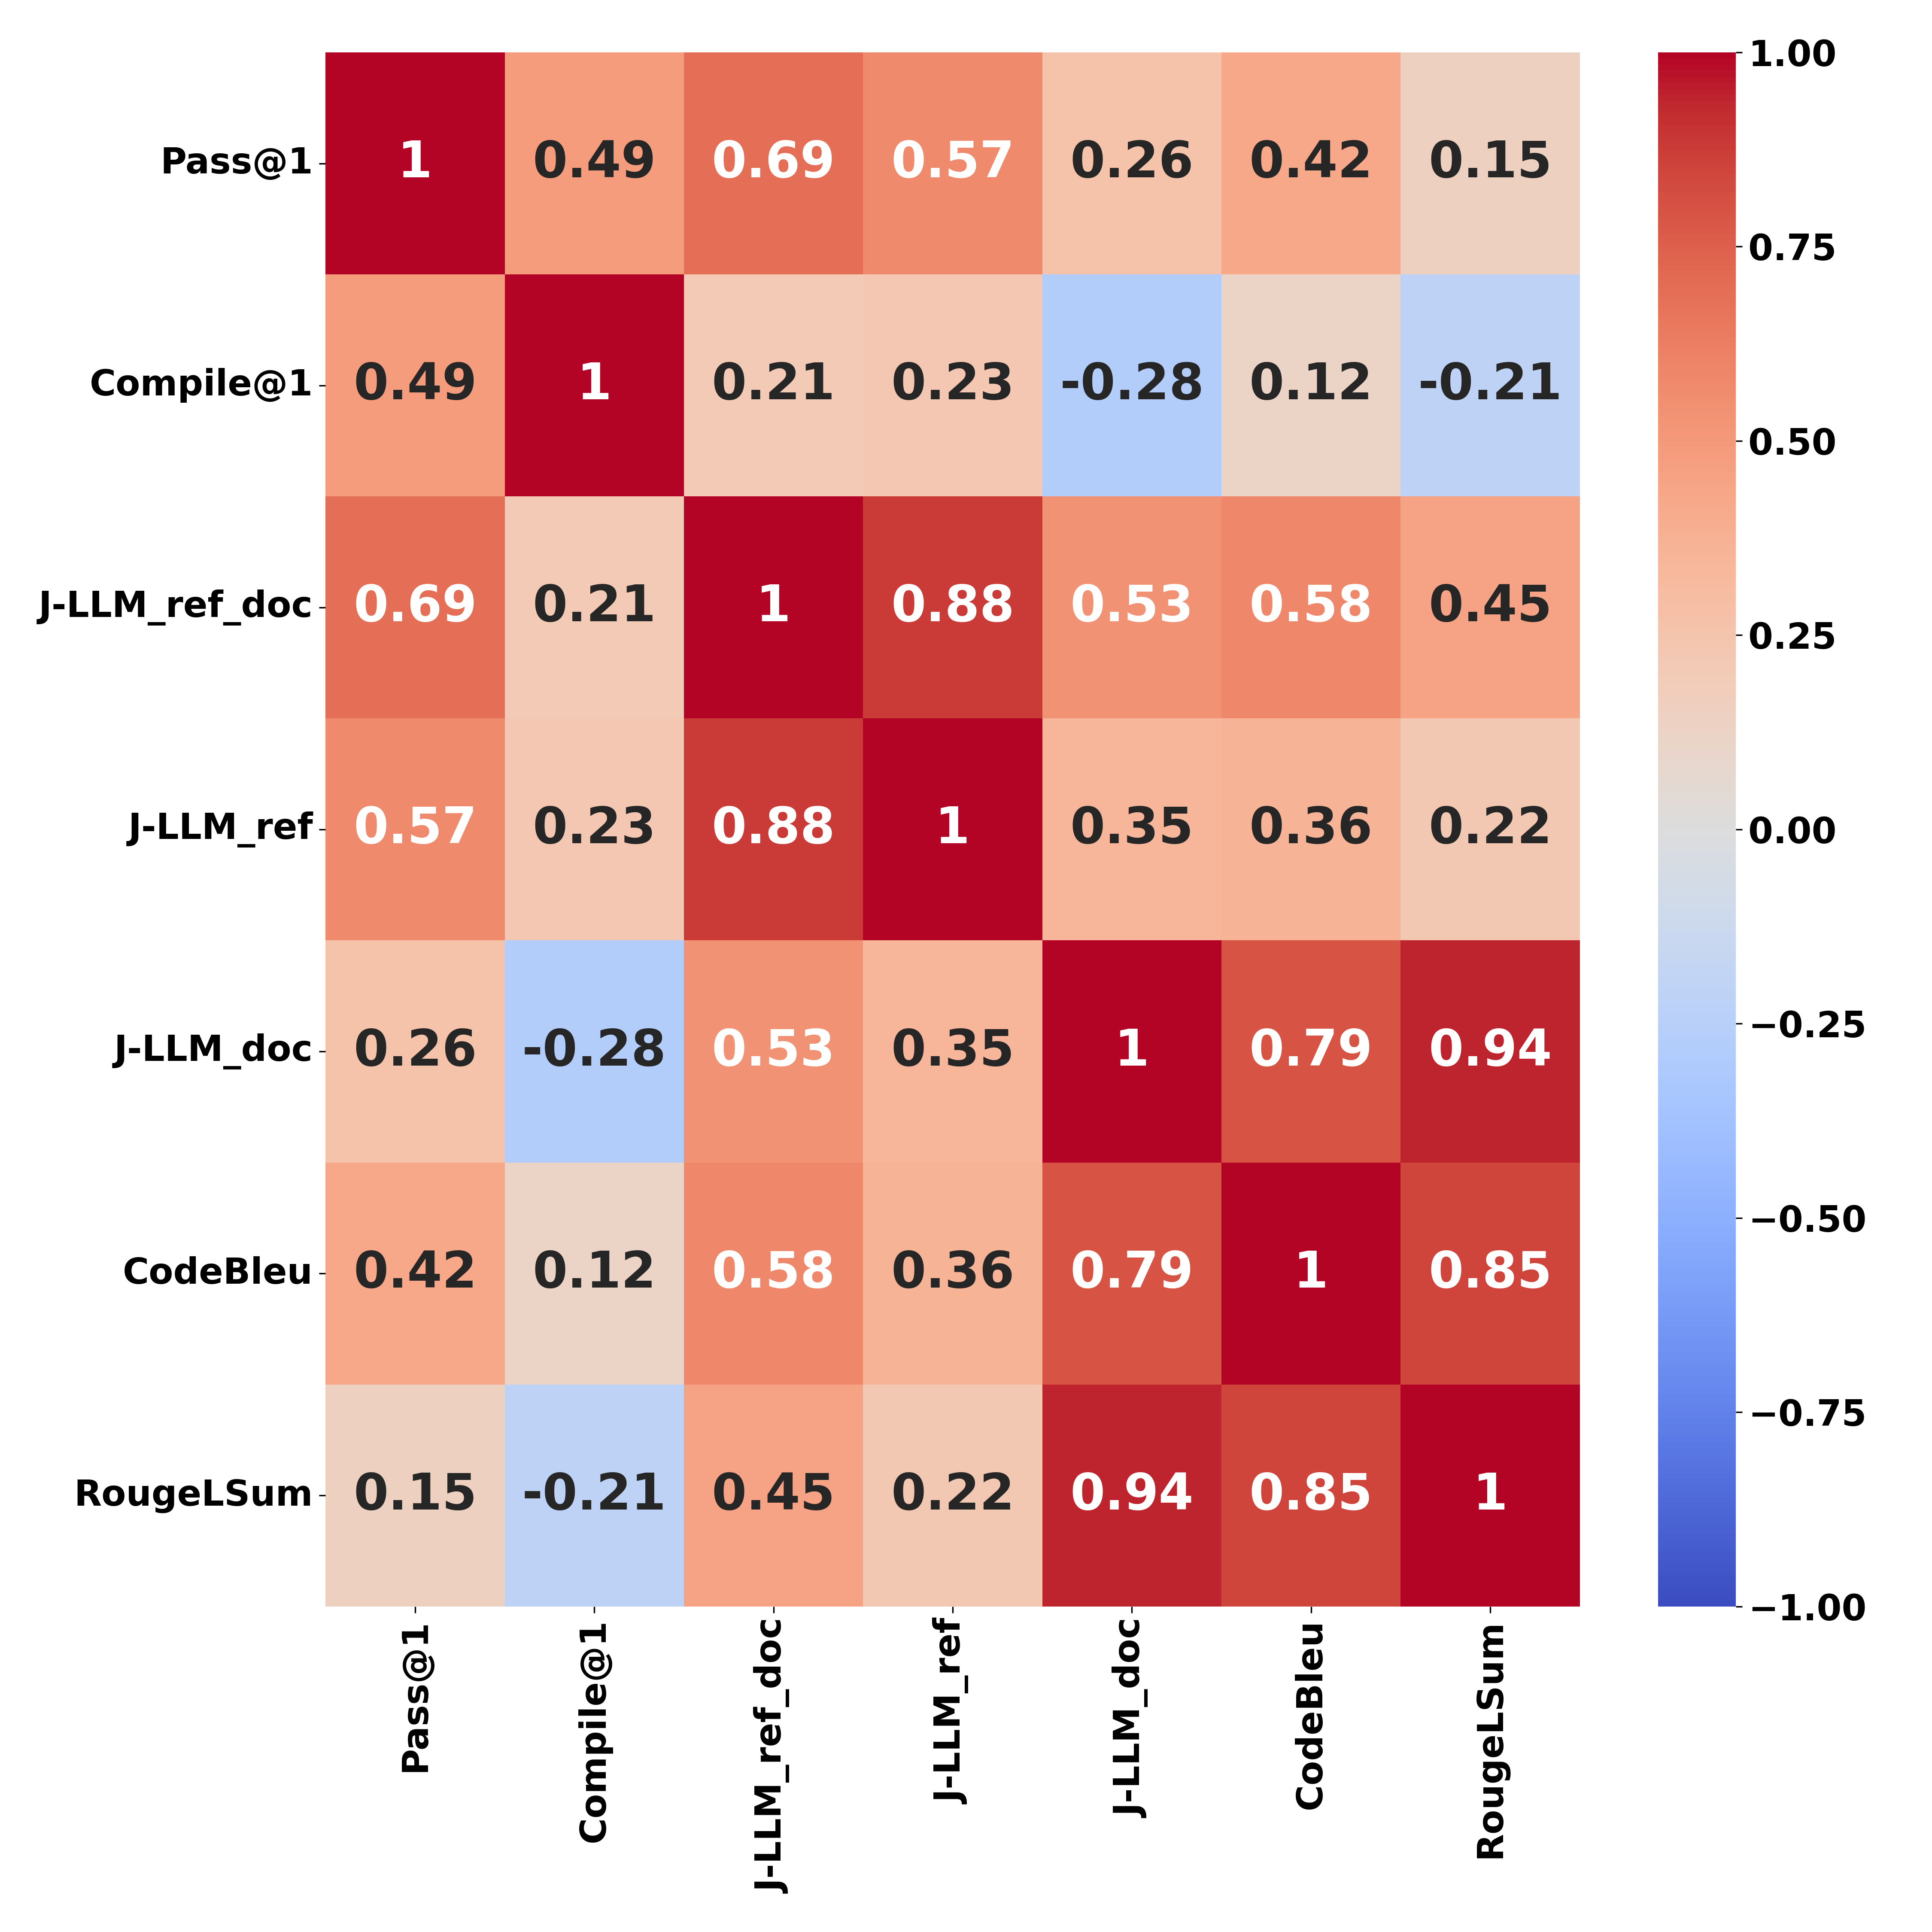
\includegraphics[width=0.48\textwidth]{images/correlation_matrix.png}
\caption{The correlation matrix of different metrics, including pass@1, compile@1, three different J-LLM instances, and the similarity scores CodeBLEU and ROUGE-LSUM.}
\label{fig:correlation_matrix}
\end{figure}

{\noindent\textbf{Threats to validity (LLM-as-a-judge bias).}}
While we observe strong cross-evaluator agreement, this does not rule out \emph{correlated} judge bias: LLM-based evaluators may share training-data priors that systematically favor particular coding styles, verbosity levels, or model families, yielding consistency that reflects shared bias rather than functional correctness. To mitigate this risk, we: (i) use a rubric-grounded judge prompt that prioritizes simulator-relevant, checkable criteria (e.g., API correctness, subsystem completeness, and required simulation-loop updates) and explicitly instructs the judge to ignore superficial stylistic signals (e.g., comment density and verbosity); (ii) assess ranking stability across multiple judge instances and verify alignment with human-expert rankings on a held-out subset from the calibration protocol; (iii) partially anchor rubric scores to execution-based outcomes (e.g., Pass@1) when available; and (iv) incorporate standard anti-bias prompt guardrails (e.g., position/length bias mitigation and structured scoring by rubric section). We additionally include a small adversarial-style check in which functionally correct but differently structured implementations are evaluated to test sensitivity to code organization. Nonetheless, judge scores should be interpreted as \emph{approximations} of functional correctness rather than proofs; further reducing residual bias remains important future work (e.g., increasing judge diversity, expanding executable test coverage, and adding complementary non-LLM automated checks such as static analysis and API-level validators).


    \begin{comment}
    \begin{table*}[t]
        \centering
        \begin{tabular}{|c|c|c|c|c|c|c|}
        \hline
        \multirow{2}{*}{Models} & \multicolumn{5}{c|}{\textbf{J-LLM\_Ref\_Doc}(1st turn, 2nd turn, 3rd turn)} & \multirow{2}{*}{\textbf{Average}} \\ \cline{2-6}
                               & MBS & FEA & VEH & SEN & RBT   &  \\ \hline
        claude-4-sonnet-20250514 & $(33, 70, 57)$ & $(37, 76, 49)$ & $(38, 61, 51)$ & $(34, 63, 41)$ & $(23, 54, 47)$ & 49 \\ \hline
o3 & $(41, 59, 65)$ & $(21, 70, 55)$ & $(26, 58, 56)$ & $(28, 51, 33)$ & $(25, 62, 46)$ & 46 \\ \hline
claude-3-7-sonnet-20250219 & $(45, 58, 58)$ & $(28, 64, 46)$ & $(25, 55, 47)$ & $(30, 34, 48)$ & $(22, 52, 40)$ & 43 \\ \hline
o4-mini & $(34, 54, 56)$ & $(28, 67, 44)$ & $(26, 48, 50)$ & $(16, 44, 42)$ & $(27, 54, 39)$ & 42 \\ \hline
qwen3-235b-a22b & $(27, 51, 51)$ & $(26, 65, 42)$ & $(19, 50, 58)$ & $(24, 51, 50)$ & $(25, 56, 38)$ & 42 \\ \hline
Gemini-2.5-pro & $(38, 52, 46)$ & $(30, 51, 53)$ & $(32, 46, 48)$ & $(28, 34, 32)$ & $(38, 64, 28)$ & 41 \\ \hline
gpt-4.1-mini & $(32, 52, 50)$ & $(27, 65, 49)$ & $(26, 54, 47)$ & $(22, 38, 38)$ & $(24, 44, 48)$ & 41 \\ \hline
gpt-4o-mini & $(17, 67, 43)$ & $(19, 69, 55)$ & $(20, 54, 56)$ & $(18, 38, 42)$ & $(19, 59, 40)$ & 41 \\ \hline
llama4-maverick & $(20, 63, 54)$ & $(20, 73, 57)$ & $(25, 50, 44)$ & $(16, 36, 34)$ & $(27, 58, 39)$ & 41 \\ \hline
llama4-scout & $(27, 58, 45)$ & $(24, 62, 47)$ & $(18, 50, 51)$ & $(20, 42, 46)$ & $(25, 61, 40)$ & 41 \\ \hline
llama-3.3-70b-instruct & $(21, 57, 59)$ & $(19, 70, 46)$ & $(20, 52, 53)$ & $(20, 44, 37)$ & $(17, 58, 40)$ & 41 \\ \hline
deepseek-r1-32b & $(23, 67, 47)$ & $(22, 70, 36)$ & $(19, 48, 46)$ & $(23, 42, 47)$ & $(20, 50, 38)$ & 40 \\ \hline
gpt-4.1-nano & $(19, 55, 52)$ & $(28, 73, 54)$ & $(20, 45, 44)$ & $(16, 51, 36)$ & $(20, 55, 39)$ & 40 \\ \hline
llama-3.1-70b-instruct & $(21, 53, 42)$ & $(17, 67, 50)$ & $(19, 49, 52)$ & $(14, 44, 47)$ & $(33, 51, 35)$ & 40 \\ \hline
gpt-4.1 & $(26, 61, 53)$ & $(23, 62, 38)$ & $(21, 60, 47)$ & $(14, 47, 36)$ & $(17, 47, 36)$ & 39 \\ \hline
Gemini-1.5-pro & $(24, 55, 49)$ & $(20, 52, 51)$ & $(19, 52, 51)$ & $(22, 52, 37)$ & $(15, 50, 33)$ & 39 \\ \hline
codestral-22b-instruct-v0.1 & $(23, 56, 51)$ & $(9, 58, 55)$ & $(12, 43, 51)$ & $(24, 47, 40)$ & $(21, 58, 38)$ & 39 \\ \hline
llama-3.1-405b-instruct & $(19, 62, 54)$ & $(20, 63, 50)$ & $(14, 48, 51)$ & $(15, 35, 49)$ & $(16, 59, 36)$ & 39 \\ \hline
mixtral-8x22b-instruct-v0.1 & $(22, 63, 48)$ & $(16, 61, 48)$ & $(21, 41, 49)$ & $(13, 50, 34)$ & $(22, 60, 42)$ & 39 \\ \hline
llama-3.1-8b-instruct & $(10, 64, 46)$ & $(13, 66, 49)$ & $(18, 46, 47)$ & $(16, 43, 36)$ & $(16, 58, 38)$ & 38 \\ \hline
mistral-nemo-12b-instruct & $(17, 49, 59)$ & $(22, 74, 51)$ & $(15, 36, 42)$ & $(22, 44, 44)$ & $(25, 37, 40)$ & 38 \\ \hline
mistral-large-latest & $(25, 60, 43)$ & $(10, 68, 45)$ & $(20, 46, 46)$ & $(26, 36, 14)$ & $(24, 56, 40)$ & 37 \\ \hline
gemma-2-27b-it & $(19, 46, 46)$ & $(25, 54, 39)$ & $(20, 52, 52)$ & $(19, 30, 30)$ & $(19, 53, 31)$ & 36 \\ \hline
mixtral-8x7b-instruct-v0.1 & $(19, 62, 43)$ & $(21, 60, 41)$ & $(17, 58, 51)$ & $(12, 31, 35)$ & $(12, 44, 33)$ & 36 \\ \hline
claude-3-5-sonnet & $(24, 41, 34)$ & $(25, 57, 45)$ & $(22, 39, 39)$ & $(27, 52, 18)$ & $(16, 44, 27)$ & 34 \\ \hline
deepseek-r1-8b & $(13, 62, 45)$ & $(13, 44, 43)$ & $(13, 39, 48)$ & $(13, 43, 45)$ & $(12, 49, 35)$ & 34 \\ \hline
gpt-4o & $(18, 47, 50)$ & $(18, 57, 38)$ & $(21, 33, 43)$ & $(22, 40, 31)$ & $(19, 46, 33)$ & 34 \\ \hline
nemotron-4-340b-instruct & $(11, 50, 39)$ & $(18, 46, 44)$ & $(20, 48, 48)$ & $(14, 36, 33)$ & $(14, 58, 31)$ & 34 \\ \hline
gemma-2-9b-it & $(24, 43, 40)$ & $(23, 43, 39)$ & $(16, 42, 49)$ & $(15, 24, 30)$ & $(22, 53, 24)$ & 32 \\ \hline
gemma-2-2b-it & $(19, 41, 39)$ & $(16, 49, 37)$ & $(11, 40, 48)$ & $(6, 33, 28)$ & $(17, 38, 34)$ & 30 \\ \hline
mamba-codestral-7b-v0.1 & $(17, 47, 49)$ & $(13, 52, 25)$ & $(13, 48, 45)$ & $(14, 18, 21)$ & $(15, 45, 27)$ & 30 \\ \hline
gemma-3-1b-it & $(11, 25, 18)$ & $(9, 30, 46)$ & $(9, 47, 43)$ & $(11, 32, 21)$ & $(14, 42, 29)$ & 26 \\ \hline
phi-3-mini-128k-instruct & $(17, 27, 32)$ & $(16, 23, 19)$ & $(17, 41, 46)$ & $(14, 14, 24)$ & $(15, 46, 22)$ & 25 \\ \hline
phi-3-medium-128k-instruct & $(10, 43, 21)$ & $(19, 24, 12)$ & $(12, 24, 34)$ & $(8, 20, 20)$ & $(13, 37, 19)$ & 21 \\ \hline
\textbf{Average} & $(23, 55, 48)$ & $(20, 59, 45)$ & $(21, 48, 49)$ & $(19, 41, 36)$ & $(21, 53, 36)$ & \textbf{38} \\ \hline
        
        \end{tabular}
        \caption{S-LLMs scores, when benchmarked with the J-LLM\_Ref\_Doc metric (values rounded to the nearest integer). These results provide a fraction of the data used to generate the results in Fig.~\ref{fig:correlation_matrix}.}
        \vspace{-10pt}
        \label{tab:llm_metrics_jllm}
        \end{table*}
    \end{comment}


\subsection{Multi-turn Analysis}

Table \ref{tab:llm_metrics_jllm} reports the multi-turn performance of S-LLMs in the SimBench environment, benchmarked with the metrics J-LLM\_Ref\_Doc. 

        \begin{table*}[htbp]
          \centering
          \resizebox{\textwidth}{!}{%
          \begin{tabular}{lcccccc}
          \toprule
          \textbf{S-LLM} & \multicolumn{5}{c}{\textbf{J-LLM Ref Doc (1st turn, 2nd turn, 3rd turn)}} & \textbf{Average} \\
          \cmidrule(lr){2-6}
          & \textbf{MBS} & \textbf{FEA} & \textbf{VEH} & \textbf{SEN} & \textbf{RBT} & \\
          \midrule
          claude-4-sonnet-20250514 & (33, 70, 57) & (37, 76, 49) & (38, 61, 51) & (34, 63, 41) & (23, 54, 47) & 49 \\
          o3 & (41, 59, 65) & (21, 70, 55) & (26, 56, 56) & (28, 51, 33) & (25, 62, 46) & 46 \\
          claude-3-7-sonnet-20250219 & (45, 58, 58) & (28, 64, 46) & (23, 56, 47) & (30, 45, 48) & (22, 52, 40) & 44 \\
          o4-mini & (34, 54, 56) & (28, 67, 44) & (26, 48, 50) & (16, 44, 42) & (27, 54, 39) & 42 \\
          qwen3-235b-a22b & (27, 51, 51) & (26, 65, 42) & (19, 50, 58) & (24, 51, 50) & (25, 56, 38) & 42 \\
          Gemini-2.5-pro & (38, 52, 46) & (30, 51, 53) & (32, 43, 48) & (28, 34, 32) & (38, 64, 28) & 41 \\
          gpt-4.1-mini & (32, 52, 50) & (27, 65, 49) & (26, 52, 47) & (22, 38, 38) & (24, 44, 48) & 41 \\
          gpt-4o-mini & (17, 67, 43) & (19, 69, 55) & (20, 52, 56) & (18, 38, 42) & (19, 59, 40) & 41 \\
          llama-3.3-70b & (21, 57, 59) & (19, 70, 46) & (20, 52, 53) & (20, 44, 37) & (17, 58, 40) & 41 \\
          llama4-maverick & (20, 63, 54) & (20, 73, 57) & (25, 50, 44) & (16, 36, 34) & (27, 58, 39) & 41 \\
          llama4-scout & (27, 58, 45) & (24, 62, 47) & (18, 50, 51) & (20, 42, 46) & (25, 61, 40) & 41 \\
          gpt-4.1-nano & (19, 55, 52) & (28, 73, 54) & (20, 45, 44) & (16, 45, 36) & (20, 55, 39) & 40 \\
          llama-3.1-70b & (21, 53, 42) & (17, 67, 50) & (19, 49, 52) & (14, 44, 47) & (33, 51, 35) & 40 \\
          Gemini-1.5-pro & (24, 55, 49) & (20, 52, 51) & (19, 52, 51) & (22, 52, 37) & (15, 50, 33) & 39 \\
          codestral-22b & (23, 56, 51) & (9, 58, 55) & (12, 43, 49) & (24, 47, 40) & (21, 58, 38) & 39 \\
          deepseek-r1-32b & (23, 67, 47) & (22, 70, 36) & (19, 48, 44) & (23, 36, 47) & (20, 50, 38) & 39 \\
          gpt-4.1 & (26, 61, 53) & (23, 62, 38) & (21, 58, 47) & (16, 47, 36) & (17, 47, 36) & 39 \\
          llama-3.1-405b & (19, 62, 54) & (20, 63, 50) & (14, 48, 51) & (15, 35, 49) & (16, 59, 36) & 39 \\
          mixtral-8x22b & (22, 63, 48) & (16, 61, 48) & (21, 41, 49) & (13, 50, 34) & (22, 60, 42) & 39 \\
          llama-3.1-8b & (10, 64, 46) & (13, 66, 49) & (18, 46, 47) & (16, 43, 36) & (16, 58, 38) & 38 \\
          mistral-nemo-12b & (17, 49, 59) & (22, 74, 51) & (15, 36, 42) & (22, 44, 44) & (25, 37, 40) & 38 \\
          mistral-large-latest & (25, 60, 43) & (10, 68, 45) & (20, 46, 44) & (26, 36, 14) & (24, 56, 40) & 37 \\
          gemma-2-27b-it & (19, 46, 46) & (25, 54, 39) & (20, 52, 52) & (19, 30, 30) & (19, 53, 31) & 36 \\
          mixtral-8x7b & (19, 62, 43) & (21, 60, 41) & (17, 58, 51) & (12, 31, 38) & (12, 44, 33) & 36 \\
          claude-3-5-sonnet & (24, 41, 34) & (25, 57, 45) & (22, 39, 39) & (27, 52, 18) & (16, 44, 27) & 34 \\
          deepseek-r1-8b & (13, 62, 45) & (13, 44, 43) & (13, 39, 48) & (13, 43, 45) & (12, 49, 35) & 34 \\
          gpt-4o & (18, 47, 50) & (18, 57, 38) & (21, 33, 43) & (22, 40, 31) & (19, 46, 33) & 34 \\
          nemotron-4-340b & (11, 50, 39) & (18, 46, 44) & (20, 48, 48) & (14, 36, 33) & (14, 50, 31) & 33 \\
          gemma-2-9b-it & (24, 43, 40) & (23, 43, 39) & (16, 42, 49) & (15, 24, 30) & (20, 53, 24) & 32 \\
          gemma-2-2b-it & (19, 41, 39) & (16, 49, 37) & (11, 40, 47) & (6, 33, 28) & (17, 38, 34) & 30 \\
          mamba-codestral-7b & (17, 47, 49) & (13, 52, 25) & (13, 48, 45) & (14, 18, 21) & (15, 45, 27) & 30 \\
          gemma-3-1b-it & (11, 25, 18) & (9, 30, 40) & (9, 47, 43) & (11, 32, 21) & (14, 42, 29) & 25 \\
          phi-3-mini-128k & (17, 27, 32) & (16, 23, 19) & (17, 41, 46) & (14, 14, 24) & (15, 46, 22) & 25 \\
          phi-3-medium-128k & (10, 43, 21) & (21, 24, 12) & (12, 24, 34) & (8, 20, 20) & (13, 37, 19) & 21 \\
          \midrule
          \textbf{Average} & (22, 53, 47) & (20, 59, 44) & (20, 47, 48) & (19, 39, 35) & (20, 51, 36) & 37 \\
          \bottomrule
          \end{tabular}
          }
          \caption{Performance of pretrained S-LLMs across five system categories (MBS, FEA, VEH, SEN, RBT) showing J-LLM Ref Doc scores for three rounds. Values in parentheses represent (1st turn, 2nd turn, 3rd turn) scores. Models are ranked by average score across all categories.}
          \vspace{-10pt}
          \label{tab:llm_metrics_jllm}
      \end{table*}
\medskip
% Section: Multi-turn Delta Analysis - Understanding Edit Capabilities
{\noindentBold{Turn-to-Turn Delta Analysis: Quantifying Edit Capabilities.}}
\label{subsec:multiturn_delta}
Iterative code modification is a critical skill in real-world development workflows. Accordingly, we analyze turn-to-turn score changes in our multi-turn evaluation to quantify how S-LLMs respond to successive modification requests. For each S-LLM -- system pair, we define:

\begin{equation}
\Delta_{12} = s_{i,2} - s_{i,1}, \quad \Delta_{23} = s_{i,3} - s_{i,2} \; ,
\end{equation}
where $s_{i,t}$ represents the J-LLM-Ref-Doc score for system $i$ at turn $t$. These deltas quantify: (1) the benefit of having existing code context ($\Delta_{12}$), and (2) the challenge of extending functionality while maintaining consistency ($\Delta_{23}$).

\textbf{Overwhelmingly positive Turn 1$\to$2 improvement.}
Table~\ref{tab:delta_global} presents the overall delta statistics across all 1,122 model-system evaluations(we have 33 S-LLMs with 34 systems). The mean $\Delta_{12} = +29.26$ is highly significant ($p < 0.001$), with \textbf{87.6\%} of cases showing improvement. This dramatic increase validates a key hypothesis: when given existing code context (Turn 2), models leverage structural information, variable naming conventions, and established patterns to produce significantly better modifications compared to generating from scratch (Turn 1). The median gain of 30 points demonstrates that this is not driven by outliers but represents a fundamental capability shift when code context is available.

\textbf{Turn 2$\to$3 reveals the difficulty of extension tasks.}
In stark contrast, $\Delta_{23} = -6.17$ is significantly negative ($p < 0.001$), with \textbf{58.5\%} of cases showing decline. This pattern reflects the increasing complexity of Turn 3 tasks, which require: (1) extending existing functionality (adding new features), (2) maintaining consistency with previous modifications, and (3) preserving correctness of unchanged components.

\begin{table}[htbp]
    \centering
    \caption{Global turn-to-turn delta statistics across 1,122 model-system pairs. All differences are highly significant ($p < 0.001$).}
    \label{tab:delta_global}
    \begin{tabular}{lcccc}
    \toprule
    \textbf{Delta} & \textbf{Mean} & \textbf{Median} & \textbf{IQR} & \textbf{Improvement \%} \\
    \midrule
    $\Delta_{12}$ & $+29.26 $ & $+30.0$ & $[13.3, 46.0]$ & 87.6\% \\
    $\Delta_{23}$ & $-6.17 $ & $-7.0$ & $[-25.0, 11.0]$ & 38.2\% \\
    \bottomrule
    \end{tabular}
\end{table}


\begin{comment}
\textbf{System category variations.}
Table~\ref{tab:delta_category} shows notable differences across simulation domains. FEA systems exhibit the largest $\Delta_{12} = +43.17$, suggesting these structural analysis tasks particularly benefit from code scaffolding (e.g., reusing mesh generation patterns, boundary condition setup). In contrast, sensor systems (SEN) show the smallest improvement ($\Delta_{12} = +19.90$), possibly because sensor configuration code is more template-driven with less opportunity for leveraging context. For $\Delta_{23}$, MBS and RBT categories show the steepest declines ($-13.29$ and $-12.55$ respectively), indicating that extending multi-body dynamics simulations poses greater challenges in maintaining kinematic consistency and preventing simulation instabilities.

\begin{table}[htbp]
    \centering
    \caption{Turn-to-turn deltas by system category. MBS: multi-body systems, FEA: finite element analysis, VEH: vehicles, SEN: sensors, RBT: robotics.}
    \label{tab:delta_category}
    \begin{tabular}{lccr}
    \toprule
    \textbf{Category} & \textbf{$\Delta_{12}$} & \textbf{$\Delta_{23}$} & \textbf{$n$} \\
    \midrule
    MBS & $+35.00 \pm 22.50$ & $-13.29 \pm 23.47$ & 245 \\
    FEA & $+43.17 \pm 25.76$ & $-0.85 \pm 22.73$ & 105 \\
    VEH & $+28.42 \pm 22.94$ & $-7.08 \pm 30.81$ & 280 \\
    SEN & $+19.90 \pm 20.39$ & $+0.61 \pm 27.32$ & 140 \\
    RBT & $+27.14 \pm 19.90$ & $-12.55 \pm 23.52$ & 210 \\
    \bottomrule
    \end{tabular}
\end{table}


\textbf{Model family differences in edit capabilities.}
Table~\ref{tab:delta_family} reveals systematic differences across model families. The Llama family demonstrates the strongest context-leveraging ability ($\Delta_{12} = +34.32$), while Phi models show the weakest ($\Delta_{12} = +16.72$), likely reflecting differences in pretraining data that include code modification examples. Interestingly, Claude models exhibit the largest Turn 2$\to$3 decline ($\Delta_{23} = -10.46$), suggesting potential overfitting to immediate context at the expense of longer-term consistency. Gemma models show the smallest decline ($\Delta_{23} = -3.57$), indicating more stable extension behavior, though their absolute performance remains lower (see Section~\ref{sec:main_results}).

\begin{table}[htbp]
    \centering
    \caption{Turn-to-turn deltas by model family (families with $n \geq 5$).}
    \label{tab:delta_family}
    \begin{tabular}{lccr}
    \toprule
    \textbf{Family} & \textbf{$\Delta_{12}$} & \textbf{$\Delta_{23}$} & \textbf{$n$} \\
    \midrule
    Llama   & $+34.32 \pm 22.57$ & $-7.02 \pm 27.44$ & 204 \\
    Mistral & $+31.27 \pm 23.50$ & $-6.43 \pm 28.11$ & 136 \\
    DeepSeek & $+31.27 \pm 23.11$ & $-7.63 \pm 30.31$ & 102 \\
    GPT     & $+30.04 \pm 20.89$ & $-6.41 \pm 25.75$ & 170 \\
    Gemma   & $+26.59 \pm 22.02$ & $-3.57 \pm 22.82$ & 136 \\
    Claude  & $+26.51 \pm 20.58$ & $-10.46 \pm 25.38$ & 102 \\
    Gemini  & $+23.66 \pm 23.70$ & $-5.65 \pm 27.09$ & 68 \\
    Phi     & $+16.72 \pm 25.80$ & $-2.28 \pm 29.17$ & 68 \\
    \bottomrule
    \end{tabular}
\end{table}
\end{comment}
\textbf{Implications for real-world deployment.}
These findings have critical implications for deploying S-LLMs in interactive development environments:

\begin{itemize}
    \item \textbf{Leverage existing code:} The substantial $\Delta_{12}$ improvements (+30 points, 87.6\% success rate) strongly advocate for always providing existing code context when requesting modifications. Tools should default to showing relevant surrounding code rather than asking models to generate modifications in isolation.
    
    \item \textbf{Manage complexity in extensions:} The consistent $\Delta_{23}$ decline (-6.2 points, 58.5\% degradation rate) suggests that large feature additions should be broken into smaller incremental steps. Rather than requesting complex multi-part extensions in a single turn, better results may come from iterative refinement with validation checkpoints.
\end{itemize}

This delta analysis indicates that SimBench probes multi-turn code editing and extension behavior, not just one-shot code generation. The resulting turn-to-turn trends—context sensitivity, extension difficulty, and category-dependent behavior, provide a diagnostic view of current S-LLM strengths and failure modes.

%\begin{figure}
%\centering
%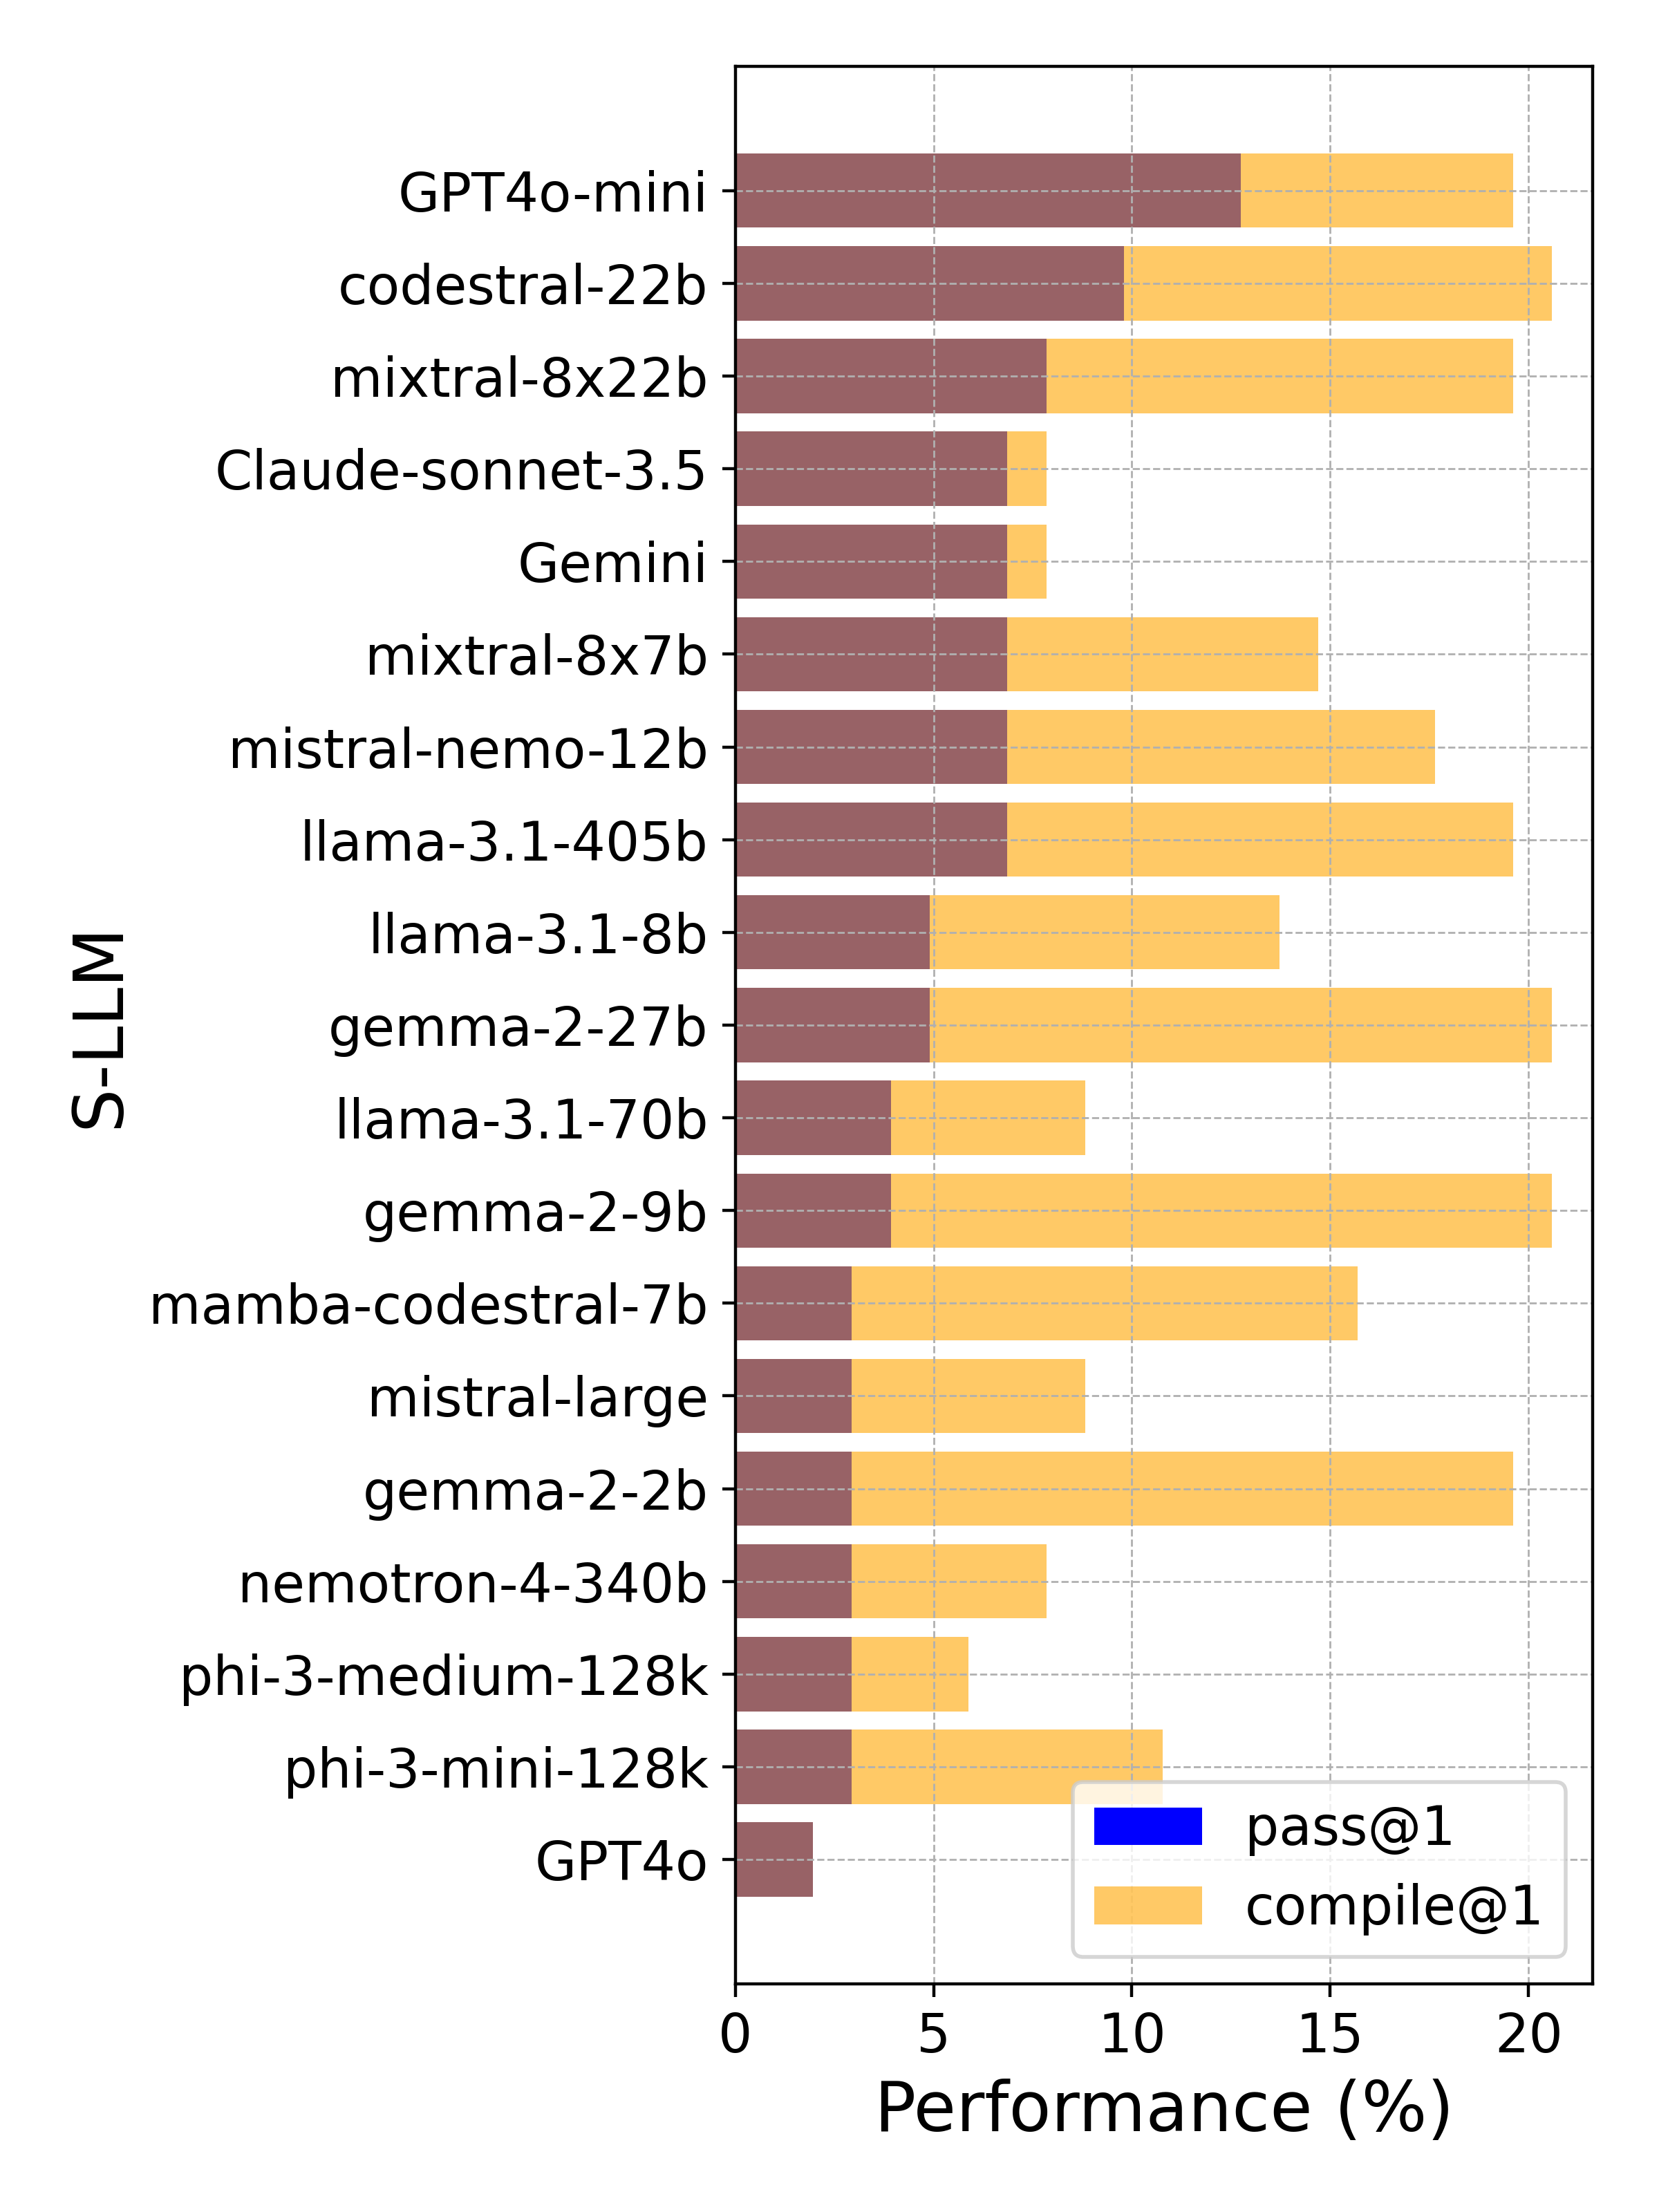
\includegraphics[width=0.4\textwidth]{images/pass_compile.png}
%\caption{The performance of S-LLMs in the SimBench environment, benchmarked with the metrics pass@1 and compile@1.}
%\end{figure}


%\begin{figure}
%\centering
%includegraphics[width=0.4\textwidth]{images/llm_scores.png}
%\caption{The performance of various S-LLMs in the SimBench environment, benchmarked with J-LLMs using three different strategies.}
%\end{figure}

\subsection{Failure Mode Analysis: System Difficulty Assessment}
\label{subsec:failure_mode}

To identify challenging scenarios and failure patterns in simulation code generation, we conduct a comprehensive system-level difficulty analysis. Table~\ref{tab:system_difficulty} presents the performance of all 34 simulation systems, ranked by overall difficulty (average J-LLM-Ref-Doc scores across all S-LLMs and all three turns). Lower scores indicate harder systems where models consistently struggle. We highlight next the lessons learned from this analysis.

\textbf{Sensor systems emerge as the most challenging domain.}
The hardest system overall is \texttt{lidar} (SEN category, overall score 23.4), which requires intricate sensor configuration including noise models, visualization pipelines, and dynamic sensor positioning. The SEN category achieves the lowest average performance (31.3), significantly below other domains. This persistent difficulty stems from:

\begin{itemize}
    \item \textbf{API complexity}: Sensor initialization requires precise parameter tuning (e.g., resolution, field-of-view, update rates) with limited error tolerance.
    \item \textbf{Visualization challenges}: Sensors demand additional rendering setup, buffer management, and frame processing that are domain-specific and poorly documented in training data.
    \item \textbf{Real-time constraints}: Sensor simulations require careful synchronization between physics updates and sensor data acquisition, a subtle requirement often missed by models.
\end{itemize}


Similarly, \texttt{camera} (SEN, 30.1) exhibits consistently low performance across all turns (T1=18.3, T2=45.8, T3=26.0), with the Turn 2$\to$3 decline (-19.7)
 highlighting the difficulty of extending sensor functionality while maintaining correct configuration. An illustrative prompt exemplifies these challenges:

\begin{quote}
\textit{Create a PyChrono simulation where a triangular mesh (loaded from a Wavefront .obj file) is visualized as a fixed body in the scene. Add a camera sensor to the body, managed by a sensor manager, with noise filters and visualizations applied to the camera images. Simulate the system, dynamically updating the camera's position in an orbit around the mesh, and print out camera buffer data at each step.}
\end{quote}

This complexity significantly contributes to lower performance metrics observed in sensor-based scenarios.

\medskip

\textbf{Robotics and vehicle systems show moderate difficulty with high variability.}
The RBT category (average 35.8) and VEH category (38.0) occupy the middle difficulty range. Systems like \texttt{vehros} (RBT, 27.8) and \texttt{sedan} (VEH, 28.6) demonstrate interesting failure patterns: relatively low Turn 1 generation scores but substantial Turn 2 improvements (+19.1 and +16.2 respectively), suggesting models can leverage context effectively once initial code structure is provided. However, the high standard deviation in these categories (e.g., \texttt{art} with std=32.1) indicates significant performance variance across different models—some handle complex kinematics well while others struggle with constraint specification.

\textbf{FEA and MBS systems are relatively easier but exhibit distinct patterns.}
The FEA category achieves the highest average performance (41.0), with \texttt{art} reaching 58.6, the easiest system overall. This success likely reflects: (1) well-structured simulation workflows with clear mesh$\to$material$\to$solver pipelines, (2) abundant finite element examples in training corpora, and (3) less ambiguity in problem specifications. The MBS category (40.8) also performs well, though systems like \texttt{cable} exhibit dramatic Turn 3 declines (-37.8), revealing challenges in extending multi-body dynamics while preserving kinematic consistency.

\textbf{Turn-specific failure modes reveal distinct challenges.}
Turn 1 (generation from scratch) proves universally difficult, with scores averaging only 20.2 and systems like \texttt{vehros} scoring just 14.7. This baseline difficulty underscores the challenge of synthesizing complete simulation setups without examples. Turn 2 (modification with context) shows dramatic improvement (average +29.3), but the benefit varies widely—from +8.7 for systems with template-like structures (minimal leverage from context) to +64.3 for complex systems where context provides critical scaffolding. Turn 3 (extension tasks) reveals brittleness: 22 out of 34 systems show performance declines, with some catastrophic drops (e.g., \texttt{cable}: -37.8) indicating models struggle to add functionality while maintaining simulation correctness.

\textbf{Implications for S-LLM development.}
While S-LLMs handle well simple, incremental edits, they still struggle with complex simulation DT generation, particularly for sensor-centric tasks. SimBench makes these limitations visible in a controlled, multi-turn setting. Ultimately, our failure mode analysis identifies three priority areas for improvement:

\begin{enumerate}
    \item \textbf{Sensor domain specialization}: Targeted training on sensor configuration patterns, visualization pipelines, and buffer management could significantly improve the weakest category.
    \item \textbf{Consistency-preserving extensions}: The widespread Turn 3 degradation calls for methods that explicitly verify backward compatibility when extending code (e.g., constraint checking, regression testing).
    \item \textbf{Variance reduction}: High inter-model variance in complex systems (robotics, vehicles) suggests ensemble or hybrid approaches might provide more reliable generation.
\end{enumerate}

These findings complement our multi-turn delta analysis (Section~\ref{subsec:multiturn_delta}), providing system-level granularity that guides both model selection for specific simulation domains and targeted improvements in S-LLM capabilities.

\begin{table}[htbp]
    \centering
    \caption{System difficulty analysis: average J-LLM-Ref-Doc scores across all S-LLMs and turns. Systems ranked by overall difficulty (lower scores indicate harder systems).}
    \label{tab:system_difficulty}
    \resizebox{0.5\textwidth}{!}{%
    \begin{tabular}{rlccccc}
    \toprule
    \textbf{Rank} & \textbf{System} & \textbf{Category} & \textbf{Turn 1} & \textbf{Turn 2} & \textbf{Turn 3} & \textbf{Overall} \\
    \midrule
    1 & lidar & SEN & 19.5 & 31.3 & 19.3 & 23.4 \\
    2 & vehros & RBT & 14.7 & 33.9 & 34.7 & 27.8 \\
    3 & sedan & VEH & 21.9 & 38.1 & 25.9 & 28.6 \\
    4 & camera & SEN & 18.3 & 45.8 & 26.0 & 30.1 \\
    5 & scm\_hill & VEH & 19.9 & 28.6 & 43.1 & 30.5 \\
    6 & veh\_app & SEN & 19.9 & 36.5 & 35.4 & 30.6 \\
    7 & m113 & VEH & 17.8 & 36.0 & 39.0 & 30.9 \\
    8 & kraz & VEH & 18.8 & 54.8 & 21.7 & 31.8 \\
    9 & scm & VEH & 22.5 & 43.7 & 32.7 & 32.9 \\
    10 & feda & VEH & 16.5 & 43.4 & 39.5 & 33.1 \\
    11 & sensros & RBT & 17.5 & 32.2 & 50.2 & 33.3 \\
    12 & pendulum & MBS & 19.7 & 39.7 & 41.0 & 33.5 \\
    13 & buckling & FEA & 21.0 & 53.2 & 28.4 & 34.2 \\
    14 & hmmwv & VEH & 21.9 & 31.5 & 50.9 & 34.8 \\
    15 & uazbus & VEH & 15.3 & 57.6 & 33.5 & 35.5 \\
    16 & handler & RBT & 20.1 & 59.5 & 27.6 & 35.7 \\
    17 & man & VEH & 20.1 & 53.1 & 34.6 & 35.9 \\
    18 & turtlebot & RBT & 20.8 & 61.6 & 29.2 & 37.2 \\
    19 & gear & MBS & 21.4 & 57.3 & 39.0 & 39.3 \\
    20 & viper & RBT & 22.6 & 66.4 & 30.2 & 39.7 \\
    21 & rigid\_multipatches & VEH & 20.7 & 35.9 & 63.7 & 40.1 \\
    22 & tablecloth & FEA & 22.3 & 51.7 & 47.6 & 40.5 \\
    23 & curiosity & RBT & 26.3 & 55.0 & 41.3 & 40.9 \\
    24 & gps\_imu & SEN & 18.6 & 44.3 & 60.5 & 41.1 \\
    25 & gator & VEH & 21.0 & 36.8 & 68.1 & 42.0 \\
    26 & cable & FEA & 21.1 & 71.7 & 33.9 & 42.3 \\
    27 & mass\_spring\_damper & MBS & 23.9 & 56.2 & 47.1 & 42.4 \\
    28 & slider\_crank & MBS & 27.2 & 52.4 & 50.2 & 43.3 \\
    29 & rotor & FEA & 19.8 & 62.8 & 48.3 & 43.6 \\
    30 & beam & FEA & 17.8 & 53.6 & 61.5 & 44.3 \\
    31 & particles & MBS & 19.6 & 61.4 & 55.3 & 45.4 \\
    32 & citybus & VEH & 19.6 & 50.4 & 67.4 & 45.8 \\
    33 & rigid\_highway & VEH & 21.2 & 63.6 & 70.0 & 51.6 \\
    34 & art & VEH & 17.9 & 82.2 & 75.8 & 58.6 \\
    \bottomrule
    \end{tabular}
    }
\end{table}

\begin{comment}
\subsection{PyChronoBench: A Multiple-Choice Benchmark for API Literacy}
\label{sec:pychronobench}

\textbf{Benchmark description.}  %
To complement the end-to-end \emph{SimBench} evaluation, we introduce
\emph{PyChronoBench}\footnote{\url{https://github.com/uwsbel/PyChronoBench}}
— a lightweight, multiple-choice benchmark that targets fine-grained
knowledge of the \texttt{PyChrono} API.  It contains \textbf{280}
diverse questions covering contact modelling, body creation, solver
settings, sensor configuration, and other frequent developer tasks.  Each
item follows the \texttt{\{instruction,input,output\}} schema and has a
single correct option among four distractors, making automatic grading
trivial. :contentReference[oaicite:0]{index=0}

\medskip
\textbf{Experimental setup.}  %
We evaluate the same pool of 20~S-LLMs used in
Section~\ref{sec:simbench-results}.  For each model we prompt once per
question (greedy decoding) and compute the \emph{Success Rate} — the
percentage of questions answered correctly.

\medskip
\textbf{Results.}  %
Table~\ref{tab:pychrono_results} lists the ten best-performing models.
A fine-tuned variant of \textbf{GPT-4o-mini} tops the chart with an
86.1\,\% success rate, closely followed by the base \textbf{GPT-4o}
(85.0\,\%).  Commercial closed-source models such as
\textbf{Claude 3.5 Sonnet} and \textbf{NemoTron-4-340B} cluster around
79\,\%.  Among open-source models, \textbf{Code\-Llama/Mamba} and the
\textbf{Llama-3.1} family exceed 74\,\%.  Raw numbers are extracted from
\texttt{success\_rates.csv} in the repository. :contentReference[oaicite:1]{index=1}

\begin{table*}[htbp]
  \centering
  \small
  \caption{Results on \textbf{PyChronoBench}: each model answers 280 multiple-choice API questions.}
  \label{tab:pychrono_results}
  \begin{tabular}{|l|c|c|c|}
    \hline
    \textbf{Model} & \textbf{Success Rate (\%)} & \textbf{Correct Matches} & \textbf{Total Questions} \\
    \hline
    GPT\mbox{-}4o\mbox{-}mini\_\textit{finetuned}                  & 86.07 & 241 & 280 \\
    GPT\mbox{-}4o (\textit{base})                                 & 85.00 & 238 & 280 \\
    Claude 4 Sonnet                                              & 82.50 & 231 & 280 \\
    Claude 3.5 Sonnet                                            & 78.93 & 221 & 280 \\
    Claude 3.7 Sonnet                                            & 76.79 & 215 & 280 \\
    NemoTron\mbox{-}4\mbox{-}340B\mbox{-}Instruct                & 78.93 & 221 & 280 \\
    CodeStral\mbox{-}22B\mbox{-}Instruct\mbox{-}v0.1             & 76.79 & 215 & 280 \\
    GPT\mbox{-}4o\mbox{-}mini (\textit{base})                    & 76.79 & 215 & 280 \\
    GPT-4.1                                                     & 75.36 & 211 & 280 \\
    GPT-4.1-Mini                                                & 74.64 & 209 & 280 \\
    GPT-4.1-Nano                                                & 71.79 & 201 & 280 \\
    Llama\mbox{-}3.1\mbox{-}405B\mbox{-}Instruct                 & 75.36 & 211 & 280 \\
    Llama\mbox{-}3.1\mbox{-}70B\mbox{-}Instruct                  & 74.64 & 209 & 280 \\
    Llama\mbox{-}3.3\mbox{-}70B\mbox{-}Instruct                  & 74.29 & 208 & 280 \\
    Llama\mbox{-}3.1\mbox{-}8B\mbox{-}Instruct                   & 71.43 & 200 & 280 \\
    Gemini-2.5 Pro                                              & 71.43 & 200 & 280 \\
    Gemini-Flash                                                 & 71.07 & 199 & 280 \\
    Gemini 1.5 Pro                                              & 70.36 & 197 & 280 \\
    Mamba\mbox{-}CodeStral\mbox{-}7B\mbox{-}v0.1                 & 70.36 & 197 & 280 \\
    DeepSeek-R1-32B                                             & 70.00 & 196 & 280 \\
    DeepSeek-R1-8B                                              & 67.86 & 190 & 280 \\
    Mixtral\mbox{-}8×22B\mbox{-}Instruct\mbox{-}v0.1             & 70.36 & 197 & 280 \\
    Mixtral\mbox{-}8×7B\mbox{-}Instruct\mbox{-}v0.1              & 66.43 & 186 & 280 \\
    Phi-3-Medium-128K-Instruct                                   & 66.07 & 185 & 280 \\
    Phi-3-Mini-128K-Instruct                                     & 65.36 & 183 & 280 \\
    Llama4 Maverick                                             & 64.64 & 181 & 280 \\
    Llama4 Scout                                                & 64.29 & 180 & 280 \\
    Gemma-2-27B-IT                                              & 63.21 & 177 & 280 \\
    Gemma-2-9B-IT                                               & 61.79 & 173 & 280 \\
    Gemma-2-2B-IT                                               & 59.29 & 166 & 280 \\
    Gemma-3-1B-IT                                               & 52.14 & 146 & 280 \\
    O3                                                          & 68.21 & 191 & 280 \\
    GPT-4o-Mini                                                 & 70.00 & 196 & 280 \\
    NEMOTRON-4-340B-Instruct (J-LLM)                             & 78.93 & 221 & 280 \\
    Codestral-22B-Instruct-v0.1 (J-LLM)                          & 76.79 & 215 & 280 \\
    Mistral-Large-Latest                                         & 66.79 & 187 & 280 \\
    Mistral-Nemo-12B-Instruct                                    & 66.43 & 186 & 280 \\
    Mamba-CodeStral-7B-v0.1 (J-LLM)                              & 65.00 & 182 & 280 \\
    Phi-3-Mini-128K-Instruct (J-LLM)                             & 60.00 & 168 & 280 \\
    Phi-3-Medium-128K-Instruct (J-LLM)                           & 55.00 & 154 & 280 \\
    \hline
  \end{tabular}
  \vspace{-8pt}
\end{table*}



\medskip
\textbf{Discussion.}  %
The rankings differ markedly from those obtained on \emph{SimBench}.
For instance, \textbf{GPT-4o} moves from the bottom of the
\emph{pass@1} leaderboard to second place on API questions, whereas its
compile-time correctness remains low.  Computing Spearman’s $\rho$ over
the overlapping models yields a negligible correlation
($\rho\!\approx\!0.06$), suggesting that low-level API literacy and
end-to-end DT generation exercise complementary capabilities.  Hence,
combining \emph{SimBench} and \emph{PyChronoBench} provides a more
rounded picture of an S-LLM’s suitability for simulation work.
\end{comment}